\section{Zielsetzung}
Der folgende Versuch beschäftigt sich mit der Funktionsweise und den Eigenschaften eines Geiger-Müller-Zählrohrs. Genauer werden die Charakteristik des Zählrohrs, die Nachentladungen und die freigesetzte Ladungsmenge untersucht, sowie die Totzeit gemessen.

\section{Theorie}
Ein Geiger-Müller-Zählrohr dient zur Messung der Intensität ionisierender Strahlung. Dies geschieht durch Absorption eines $\alpha$- oder $\beta$-Teilchens, bzw. eines $\gamma$- oder Röntgenquants, welche einen elektrischen Impuls auslösen können, der gemessen
werden kann.

Zum Aufbau des Zählrohrs(s. Abbildung \ref{fig:aufbaurohr}) gehört ein mit einem Gasgemisch gefüllter Kathodenzylinder mit dem Radius $r_{\text{k}}$, in dem sich ein Draht mit dem Radius $r_{\text{a}}$ befindet. Wird eine Spannung $U$ angelegt, so dient der Draht als Anode und es entsteht ein
radialsymmetrisches elektrisches Feld, dessen Feldstärke von $U$, den Radien, sowie dem Abstand $r$ von der Zählrohrachse abhängt:

\begin{equation*}
E(r) = \frac{U}{r\cdot \text{ln}(\frac{r_{\text{k}}}{r_{\text{a}}})}.
\end{equation*}
Die Beschleunigung eines geladenen Teilchens in diesem E-Feld ist umso größer, je dünner der Anodendraht ist.

\begin{figure}[h!tbp]
	\centering
	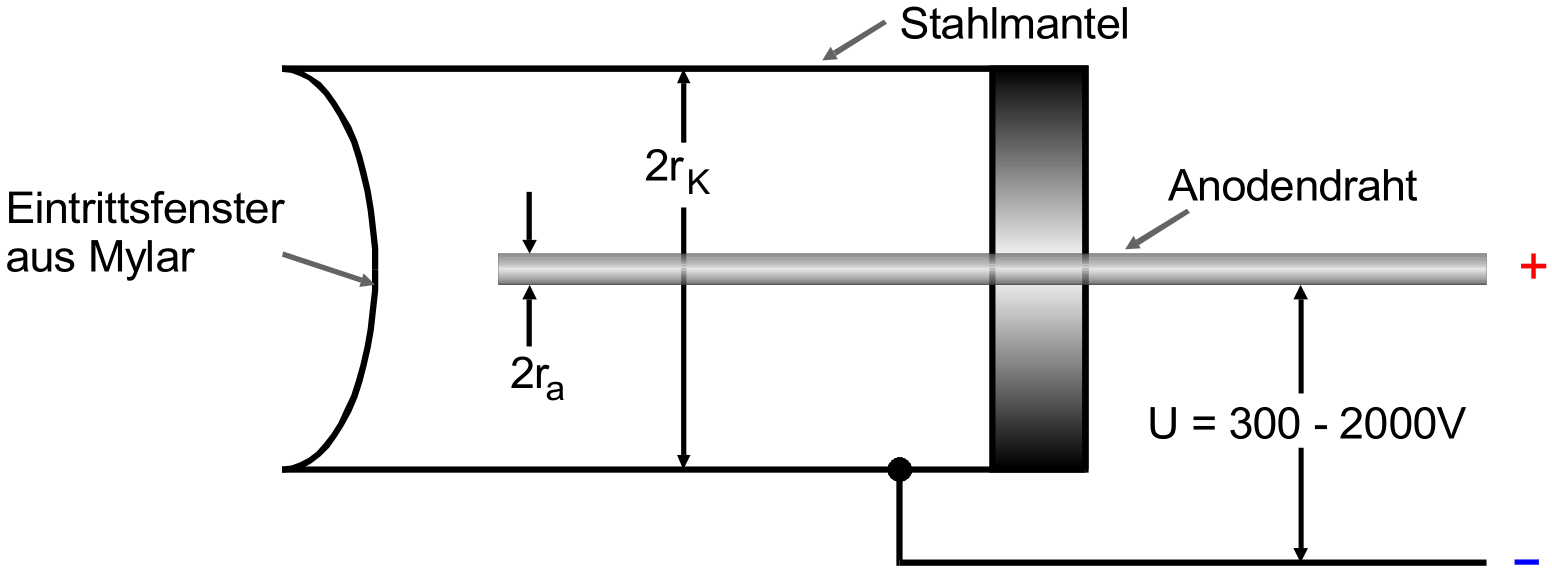
\includegraphics[width=0.8\linewidth]{../../aufbaurohr}
	\caption{Aufbau eines Endfenster-Zählrohrs, \cite[1]{anleitung703}. }
	\label{fig:aufbaurohr}
\end{figure}

Wenn ein geladenes Teilchen in das Zählrohr gelangt, so kommt es zu Ionisationsakten mit dem Gas, wodurch das geladene Teilchen seine kinetische Energie verliert. Durch die Ionisation entstehen Elektronen und positive Ionen, wobei deren Anzahl proportional
zu der Energie ist, die das geladene Teilchen besitzt. Die Elektronen bewegen sich durch das elektrische Feld zur Anode hin, wobei die angelegte Spannung berücksichtigt werden muss. Es wird die Abbildung \ref{fig:bereiche} in Betracht genommen, da das Verhalten des Zählrohrs von der angelegten Spannung abhängt:

\begin{itemize}
	\item Bei geringen Spannungen erreichen nicht alle erzeugten Elektronen den Draht, da sich ein Teil von ihnen wieder rekombiniert und damit nicht zu den zu messenden Impulsen beiträgt.
	\item Wird die Spannung erhöht, so sinkt die Wahrscheinlichkeit, dass sich die Elektronen rekombinieren. Mit höheren Spannungen kommen also alle Elektronen an der Anode an. Da die Anzahl der entstehenden Elektronen proportional zur Energie und der 
	Intensität der Strahlung ist, ist auch der Ionisationsstrom proportional zu diesen Größen. In diesem Fall wird das Zählrohr Ionisationskammer genannt, die aufgrund der geringen Ströme nur bei hoher Strahlungsintensität verwendet werden kann.
	\item Bei noch höheren Spannungen kommt es zur sogenannten Townsend-Lawine. Nehmen die Elektronen durch die Stöße mit den Gas-Atomen Energie auf, so sind sie in der Lage ebenfalls ionisieren zu können. Damit nimmt die Anzahl der Elektronen 
	kaskadenförmig zu. Die auf das Zählrohr abgegebene Ladung $Q$ ist groß genug um gemessen werden zu können. Durch ihre Proportionalität zur Energie, die von den geladenen Teilchen stammt, kann man in diesem Spannungsbereich auch die Energie messen.
	In diesem Fall wird das Messinstrument Proportionalitätszählrohr genannt.
	\item Bei Spannungen über dem Proportionalitätsbereich beginnt der Auslösebereich, welcher auch der Arbeitsbereich des Geiger-Müller-Zählrohrs ist. Hier kommt es bei der Elektronenkaskade zur Entstehung von UV-Protonen, die sich auch senkrecht zum 
	E-Feld bewegen können und imstande sind im gesamten Zählrohr weitere Elektronenlawinen auszulösen. Die Ladung, die sich am Anodendraht ansammelt ist nicht mehr von der Primärionisation abhängig sondern vom Volumen des Rohrs und der Spannung $U$ und
	kann gut gemessen werden.
	
\end{itemize}

\begin{figure}[h!tbp]
	\centering
	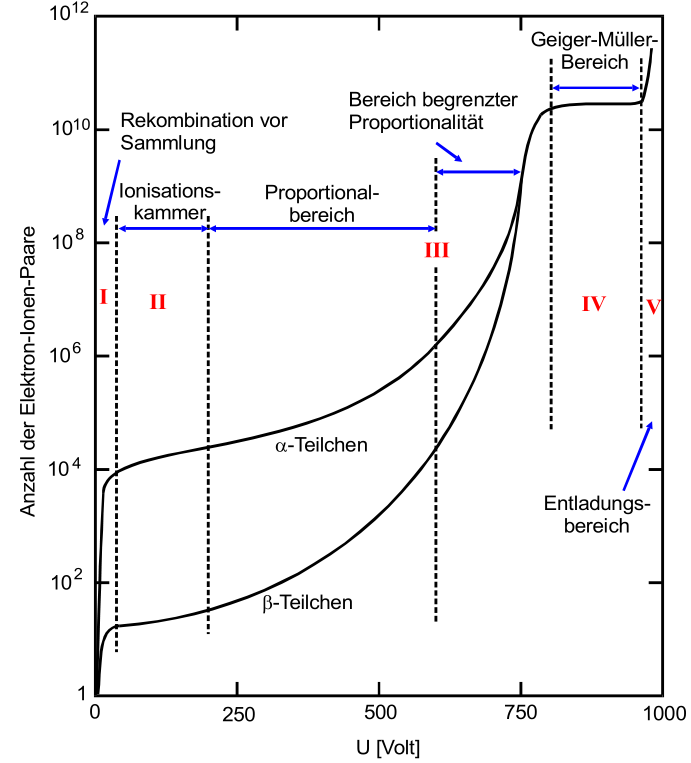
\includegraphics[width=0.8\linewidth]{../../bereiche}
	\caption{Anzahl der Elektronen-Ionenpaare in Abhängigkeit von der Spannung, \cite[2]{anleitung703}.}
	\label{fig:bereiche}
\end{figure}

\newpage
Zu den wichtigen Größen des Geiger-Müller-Zählrohrs gehören die Tot- und Erholungszeit, sowie die Nachentladungen. Wesentlich sind hier die positiven Ionen, die mit den Elektronen zusammen entstehen. Da die Ionen schwerer sind als die Elektronen, bewegen 
sie sich länger im Gasraum und bilden eine temporäre, radialsymmetrische, positive Raumladung, die Ionenschlauch genannt wird. Diese schwächt das elektrische Feld für die Zeit $T$ in der Umgebung des Drahtes ab, sodass es zu keinen Stoßionisationen mehr kommen 
kann.  Daraus folgt, dass während der Zeit $T$ keine elektrischen Impulse mehr gemessen werden können, weshalb $T$ Totzeit genannt wird. Sobald sich die positive Raumladung zum Mantel des Zählrohrs bewegt, nimmt die Feldstärke zu und es können wieder 
eintreffende Teilchen registriert werden. Sobald die Ionenwolke neutralisiert wurde, besitzt das Feld seine ursprüngliche Stärke und auch die Zahl der Ladungsimpulse $Q$ erreicht wieder ihren Ausgangswert. Die Zeit nach der Totzeit, während der die Impulse eine 
geringere Höhe haben, wird als Erholungszeit $T_{\text{E}}$(s. Abbildung \ref{fig:zeiten}) bezeichnet.

\begin{figure}[h!tbp]
	\centering
	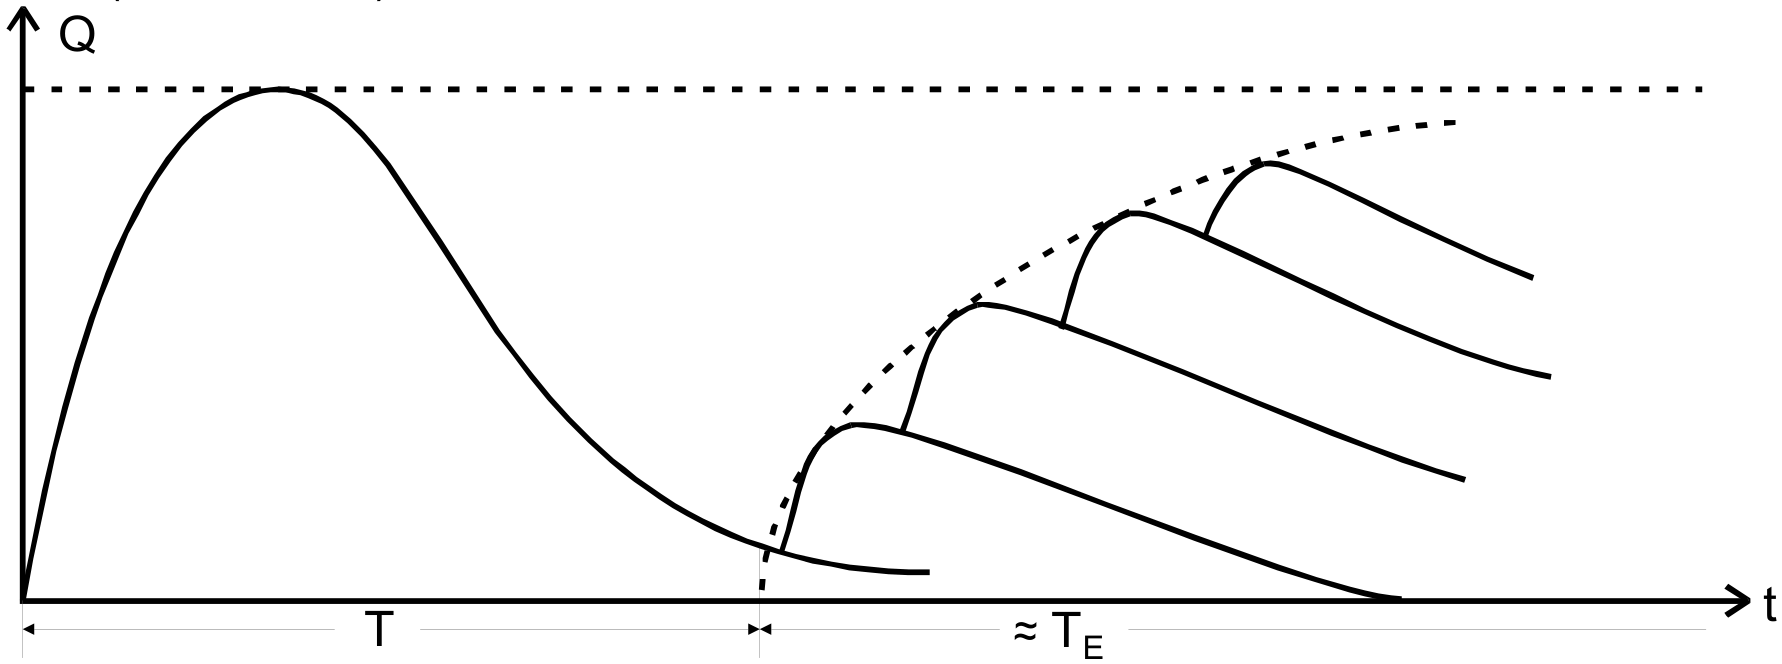
\includegraphics[width=0.8\linewidth]{../../zeiten}
	\caption{Tot- und Erholungszeit im Ladungs-Zeit-Diagramm, \cite[3]{anleitung703}.}
	\label{fig:zeiten}
\end{figure}

Wenn die Ionen am Mantel neutralisiert werden, so können sie durch Übertragung ihrer Energie Elektronen aus dem Material lösen. Diese Sekundärelektronen können wiederum zusätzliche Impulse auslösen, die Nachentladungen heißen. Weil ihre Laufzeit $T_{\text{L}}$
größer ist als die Totzeit $T$ sollen Nachentladungen vermieden werden, da sie nicht vom Durchgang von ionisierenden Teilchen zu unterscheiden sind und dadurch die Zahl der eigentlichen Impulse verfälscht wird. Aus diesem Grunde wird ein Alkoholdampf in das
Zählrohr gegeben, damit die positiven Ionen mit ihrer Energie keine Elektronen aus dem Metallmantel herausschlagen können, sondern stattdessen zu Schwingungen angeregt werden. Damit werden vom Zählrohr nur noch Impulse durch einfallende Teilchen aufgenommen.

Wird die registrierte Teilchenzahl $N$ gegen die angelegte Spannung $U$ aufgetragen, wobei die Strahlungsintensität konstant gehalten wird, so ergibt sich eine Kurve, die Charakteristik genannt wird.

\begin{figure}[h!tbp]
	\centering
	\includegraphics[width=0.7\linewidth]{zahlrohr}
	\caption{Zählrohrcharakteristik, \cite[5]{anleitung703}.}
	\label{fig:zahlrohr}
\end{figure}


Ab einer Spannung $U_{\text{E}}$ beginnt der lineare Teil des Kurvenverlaufs, der Plateau genannt wird und gleichzeitig der Arbeitsbereich des Zählrohrs ist. Das Plateau hat im Idealfall die Steigung Null, in der Realität ist jedoch durch eine geringe Zunahme 
von $N$ eine leichte Steigung zu beobachten. Grund dafür sind Nachentladungen, die auch trotz des Alkoholdampfs auftreten. Eine geringe Steigung und ein längerer Verlauf des Plateaus sprechen für ein qualitatives Zählrohr. Zum Ende hin nimmt die Anzahl der 
Nachentladungen schlagartig zu, dieser Bereich ist der Bereich der Dauerentladungen. 

Als Ansprechvermögen wird die Wahrscheinlichkeit bezeichnet, dass ein einfallendes Teilchen im Geiger-Müller-Zählrohr nachgewiesen wird. Für $\alpha$- und $\beta$-Teilchen beträgt diese Wahrscheinlchkeit fast 100\%, bei Photonen allerdings liegt das
Ansprechvermögen bei etwa 1\%. Um zu erreichen, dass die Teilchen in das Zählrohrvolumen gelangen können, wird eine Endfensterröhre eingesetzt. Bei dieser besteht die Stirnseite aus einem Material mit Atomen kleiner Ordnungszahl, durch die die geladenen Teilchen 
leicht hindurchtreten können. 